\documentclass[aspectratio=169,11pt]{beamer}
\usepackage[T1]{fontenc}
\usepackage{lmodern}
\usepackage{booktabs}
\usepackage{tikz}
\usetikzlibrary{arrows.meta,positioning}
\definecolor{Navy}{HTML}{17324D}
\definecolor{Teal}{HTML}{007F7B}
\definecolor{Gold}{HTML}{BA741B}
\definecolor{Soft}{HTML}{EEF3F6}
\definecolor{Muted}{HTML}{586879}
\setbeamercolor{normal text}{fg=Navy,bg=white}
\setbeamercolor{frametitle}{fg=Navy}
\setbeamercolor{structure}{fg=Teal}
\setbeamercolor{block title}{fg=white,bg=Teal}
\setbeamercolor{block body}{fg=Navy,bg=Soft}
\setbeamerfont{frametitle}{size=\Large,series=\bfseries}
\setbeamertemplate{navigation symbols}{}
\setbeamersize{text margin left=8mm,text margin right=8mm}
\setbeamertemplate{footline}{\hspace{8mm}\scriptsize\color{Muted}Exploratory research\hfill 11 September 2026\hspace{6mm}\insertframenumber/\inserttotalframenumber\hspace{8mm}\vspace{3mm}}
\setbeamertemplate{frametitle}{\vspace{3mm}\insertframetitle\par\vspace{2mm}}
\newcommand{\smallnote}[1]{\vfill{\scriptsize\color{Muted}#1\par}}
\newcommand{\takeaway}[1]{\begin{beamercolorbox}[sep=2.5mm,wd=\linewidth]{block body}#1\end{beamercolorbox}}
\tikzset{card/.style={draw=Teal,rounded corners=2mm,fill=Soft,align=center,inner sep=3mm},flow/.style={-{Stealth[length=2mm]},thick,draw=Teal}}
\hypersetup{pdftitle={Teaching a small language model to divide and combine work},pdfauthor={Alex Towell},colorlinks=true,urlcolor=Teal}

\begin{document}

\begin{frame}[t]
\frametitle{Can a small model solve harder problems\\by dividing the work?}
\vspace{4mm}
{\large Preliminary research and questions for discussion}\par
\vspace{8mm}
\begin{columns}[T,onlytextwidth]
\begin{column}{0.48\textwidth}
\begin{block}{We can teach a useful routine.}
Training improved how the model gathers information and calculates an answer.
\end{block}
\end{column}
\begin{column}{0.48\textwidth}
\begin{block}{The connections also matter.}
A good answer to a small question can be lost or misused when answers are combined.
\end{block}
\end{column}
\end{columns}
\vspace{5mm}
Our next goal is to turn these observations into a narrow, reproducible research contribution.
\smallnote{Alex Towell \quad | \quad Advisor discussion \quad | \quad These are preliminary findings, not a general solution.}
\end{frame}

\begin{frame}[t]
\frametitle{An RLM gives the model a workspace\\and a way to ask smaller questions.}
\centering
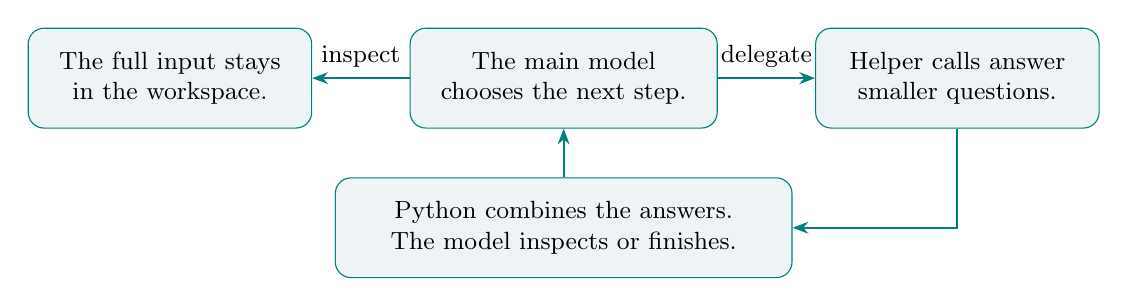
\begin{tikzpicture}[font=\small]
\node[card,text width=3.0cm] (data) at (0,0) {The full input stays\\in the workspace.};
\node[card,text width=3.3cm] (root) at (5,0) {The main model\\chooses the next step.};
\node[card,text width=3.0cm] (helpers) at (10,0) {Helper calls answer\\smaller questions.};
\node[card,text width=5.2cm] (result) at (5,-1.9) {Python combines the answers.\\The model inspects or finishes.};
\draw[flow] (root) -- node[above]{inspect} (data);
\draw[flow] (root) -- node[above]{delegate} (helpers);
\draw[flow] (helpers.south) |- (result.east);
\draw[flow] (result.north) -- (root.south);
\end{tikzpicture}
\par\vspace{4mm}
\raggedright
The main model need not read every record itself. A helper can divide its own task again.
\smallnote{RLM means recursive language model. Our tests mostly use one layer of helper calls.\par
Concept: \href{https://alexzhang13.github.io/blog/2026/harness/}{Alex Zhang's blog} and \href{https://arxiv.org/abs/2512.24601}{Recursive Language Models}.}
\end{frame}

\begin{frame}[t]
\frametitle{The helper reads the text; Python does the counting.}
\takeaway{For each user, add the weights of their place questions. How many users have a total above 5?}
\vspace{3mm}
\centering
\renewcommand{\arraystretch}{1.12}
\begin{tabular}{llrc}
\toprule
User & Question & Weight & Place question? \\
\midrule
Ada & Where is Oslo? & 4 & Yes \\
Ada & What is the capital of Peru? & 3 & Yes \\
Ben & Who wrote Hamlet? & 6 & No \\
Ben & Where is Kyoto? & 2 & Yes \\
\bottomrule
\end{tabular}
\par\vspace{3mm}
{\large Python computes Ada: $4+3=7$ and Ben: $2$.\par
\vspace{2mm}Only Ada exceeds 5, so the answer is \textcolor{Teal}{\textbf{1 user}}.}
\smallnote{Simplified illustration, not a quoted training example. Text-reading errors and calculation errors are different.}
\end{frame}

\begin{frame}[t]
\frametitle{We trained the model on examples of actions,\\not just final answers.}
\begin{columns}[T,onlytextwidth]
\begin{column}{0.48\textwidth}
\begin{block}{What the model observes}
The question, a path to the records, and basic information about the input.
\end{block}
\vspace{2mm}
\begin{block}{What it observes next}
The helper's actual labels and the result returned by Python.
\end{block}
\end{column}
\begin{column}{0.48\textwidth}
\begin{block}{What the example teaches it to do}
Read the records and ask the helper to classify them.\par\medskip
Choose the calculation that this question requires.\par\medskip
Run that calculation and return its answer.
\end{block}
\end{column}
\end{columns}
\vspace{1mm}
Supervised fine-tuning (SFT) teaches demonstrated actions. Our data use public questions with added users and weights.
\smallnote{72 demonstrations; six passes through all 72. Helper mistakes were preserved. We trained a small set of added weights, not the full model. This is a starting skill, not open-ended planning.}
\end{frame}

\begin{frame}[t]
\frametitle{Training gains appeared again\\with a different set of demonstrations.}
\centering
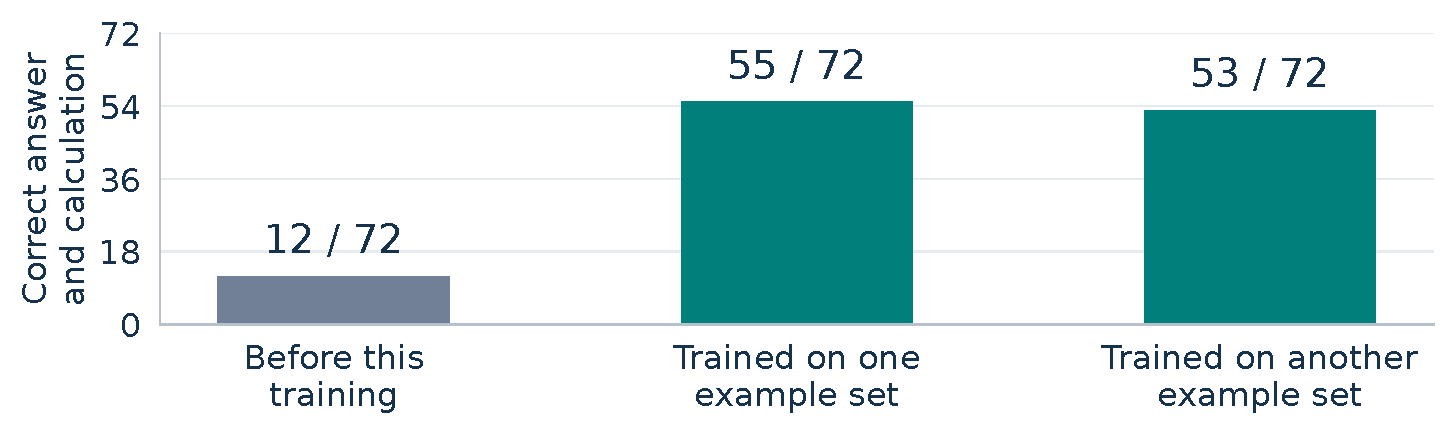
\includegraphics[width=0.91\textwidth]{figures/training.pdf}
\par\vspace{1mm}
\raggedright
Success means a correct answer from the requested calculation, not a lucky match.
\smallnote{Both runs restart from the same already-trained model; the third bar is not more training on the second. All use the same 72 questions, with changed names and numbers, on eight previously used inputs. Missing results: 17, 0, and 2. Even counting all missing baseline results as successes gives only 29. [S1, S2]}
\end{frame}

\begin{frame}[t]
\frametitle{An answer can be right for the wrong record.}
\begin{columns}[T,onlytextwidth]
\begin{column}{0.57\textwidth}
\begin{block}{A simple reading task}
Passage: ``Maya bought a red bike.''\par\medskip
Row 7: ``Maya bought a vehicle.''\par
The passage supports this statement.\par\medskip
Row 8: ``The bike is blue.''\par
The passage contradicts this statement.
\end{block}
\end{column}
\begin{column}{0.39\textwidth}
\begin{block}{What if the answer slot for row 7 carries row 8's ID?}
The model may answer for row 8 instead.\par\medskip
``Contradicted'' is then a sensible label---attached to the wrong statement.
\end{block}
\end{column}
\end{columns}
\vspace{4mm}
In our test, misleading record IDs reduced accuracy from about 80\% to 39\%.
\smallnote{The example is illustrative. In the actual 16-batch test, unrelated IDs gave 618/768 correct labels; IDs pointing to another visible record gave 298/768. Output IDs were forced by the format; the model chose the labels. This is evidence about behavior, not a proven internal mechanism. [Evidence H1]}
\end{frame}

\begin{frame}[t]
\frametitle{Matching row numbers on both sides\\helped the model keep answers aligned.}
\centering
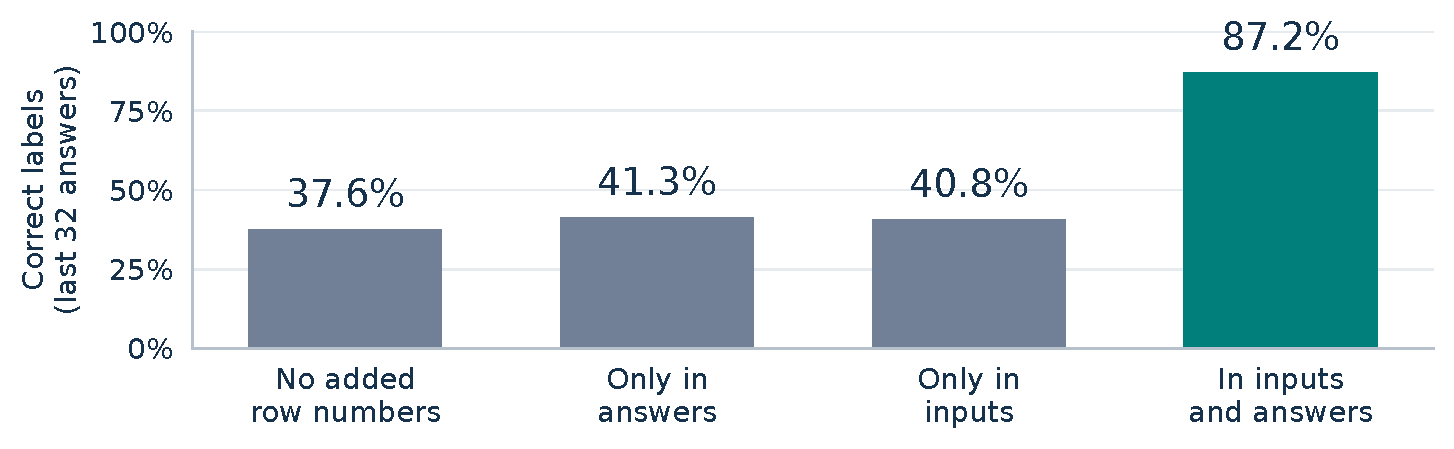
\includegraphics[width=0.91\textwidth]{figures/row-matching.pdf}
\par\vspace{1mm}
\raggedright
The benefit of matching both sides was positive in all 16 new batches.
\smallnote{We measured the later 32 of 48 statements, across three identifier conditions: 1,536 labels per bar. Batches, not repeated labels, are independent units. The format supplies the keys, not the answers. [H2]}
\end{frame}

\begin{frame}[t]
\frametitle{Matching tags helped both tested models,\\and the tags did not have to be numbers.}
\centering
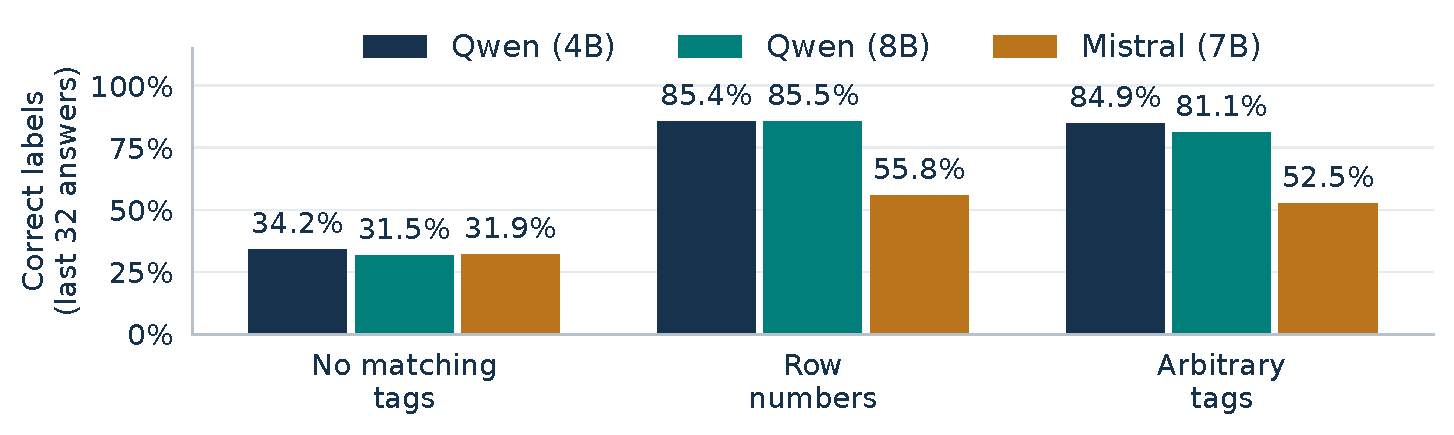
\includegraphics[width=0.91\textwidth]{figures/cross-model-keys.pdf}
\par\vspace{1mm}
\raggedright
Ordinary numbers led for the larger model, but arbitrary tags also helped.
\smallnote{Two Qwen models, same 16 batches; 1,536 later labels per bar. Both gains appeared in every batch for both models. The software supplied tags and order, not labels. This does not isolate size or test a different model family. [H3, H4]}
\end{frame}

\begin{frame}[t]
\frametitle{Better individual labels did not reliably\\produce the right combined answer.}
\centering
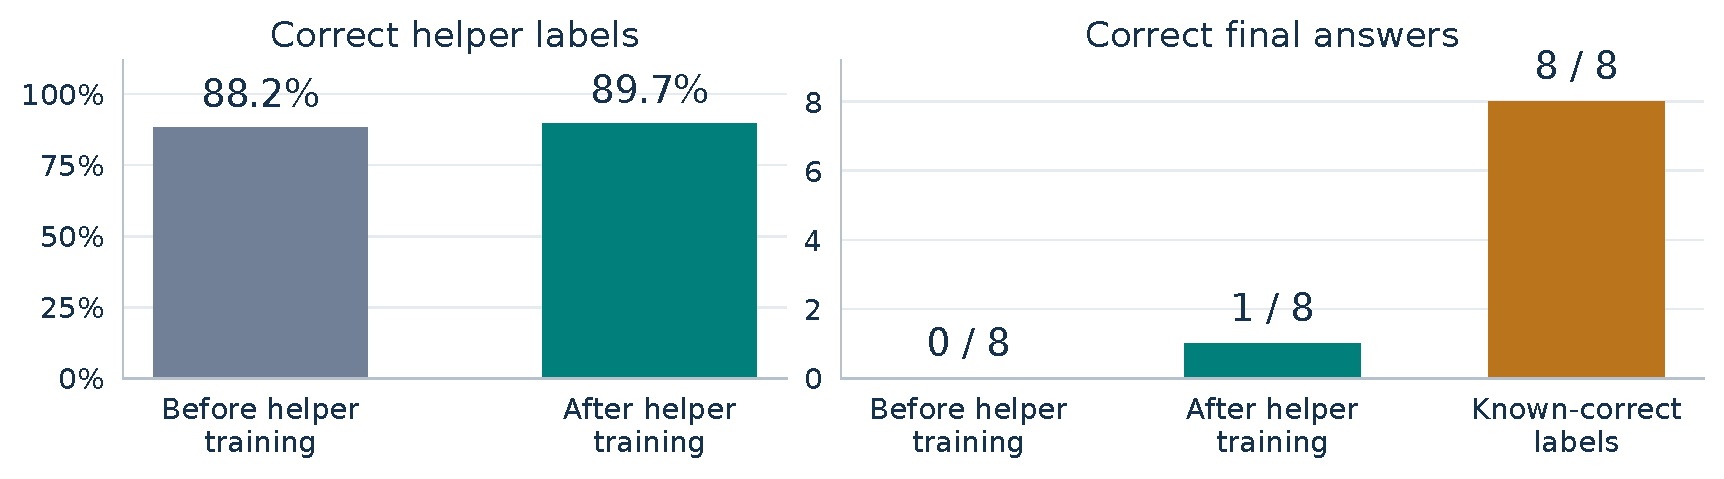
\includegraphics[width=0.99\textwidth]{figures/composition.pdf}
\par\vspace{2mm}
\raggedright
Here we trained the helper. The plan and Python calculation were supplied.
\smallnote{1,280 label slots; eight problems sharing four inputs. Reference labels are a diagnostic control, not information given to the model. Overall numerical error did not improve. [C1]}
\end{frame}

\begin{frame}[t]
\frametitle{This reward-training recipe\\did not improve the trained model.}
We also let the model try solutions and rewarded correct final answers.\par
\vspace{5mm}
\begin{columns}[T,onlytextwidth]
\begin{column}{0.47\textwidth}
\begin{block}{Before reward training}
\centering\vspace{3mm}{\Huge 55 / 72}\par\vspace{3mm}
Verified correct final answers.
\end{block}
\end{column}
\begin{column}{0.47\textwidth}
\begin{block}{After six weight updates}
\centering\vspace{3mm}{\Huge 47 / 72}\par\vspace{3mm}
Verified correct final answers.
\end{block}
\end{column}
\end{columns}
\vspace{5mm}
This changes our next experiment, not our view of whether reward training can ever work.
\smallnote{This is a different readout and metric from slide 5: final-answer correctness alone. Missing results cannot reverse the decline (before: 55--56 possible; after: 47--50). One small model, one recipe, and a previously used panel. We will test a smaller update size and better ways to assess intermediate work. [Evidence R1]}
\end{frame}

\begin{frame}[t]
\frametitle{The next experiments should test\\whether these gains survive a harder setting.}
\begin{block}{For the training result}
Test the two trained models on new inputs and unfamiliar ways of combining the smaller tasks.
\end{block}
\vspace{1mm}
\begin{block}{For the input--answer matching result}
Test whether matching tags also improve the final combined answer. Then try a different task or model family.
\end{block}
\vspace{2mm}
\takeaway{A strong paper should explain when the improvement works and where it stops.}
\smallnote{These are next tests, not findings. Numbered batch prompts already exist; our contribution must go beyond ``numbering helps.''}
\end{frame}

\begin{frame}[t]
\frametitle{The longer-term goal is to learn\\how to investigate and divide a new problem.}
\centering
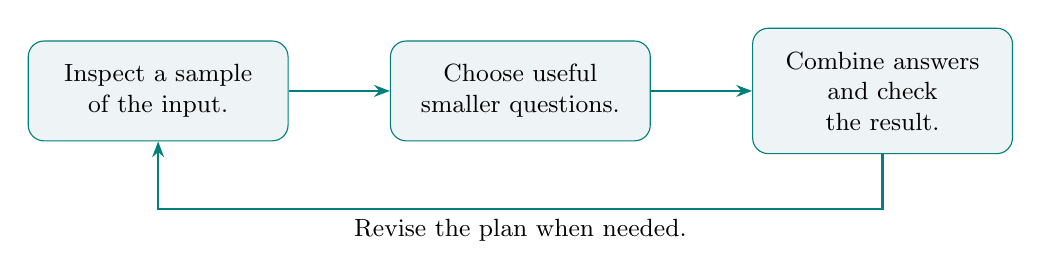
\begin{tikzpicture}[font=\small]
\node[card,text width=2.7cm] (a) at (0,0) {Inspect a sample\\of the input.};
\node[card,text width=2.7cm] (b) at (4.6,0) {Choose useful\\smaller questions.};
\node[card,text width=2.7cm] (c) at (9.2,0) {Combine answers\\and check the result.};
\draw[flow] (a)--(b);
\draw[flow] (b)--(c);
\draw[flow] (c.south) -- ++(0,-0.7) -| node[below,pos=0.25]{Revise the plan when needed.} (a.south);
\end{tikzpicture}
\par\vspace{10mm}
\raggedright
We can start with examples, then learn from checked outcomes. We can also improve the tools and instructions alongside the model.
\smallnote{This is a research direction, not an achieved capability. The related rlm-bootstrap project supplies ideas for this learning loop. Future comparisons must separate improvements in the model from improvements in its tools.}
\end{frame}

\begin{frame}[t]
\frametitle{Which result should we turn into\\the next focused study?}
\vspace{1mm}
\begin{block}{What would make the finding convincing?}
Should we prioritize a second model, a different task, or a clearer explanation of the failure?
\end{block}
\vspace{2mm}
\begin{block}{Where would this matter most?}
Is there a realistic task in your work where many small judgments must be combined reliably?
\end{block}
\vspace{2mm}
Our current recommendation is to connect the strong input--answer matching result to a useful final-task improvement.
\smallnote{The guide explains each slide. Companion documents give methods, unsuccessful experiments, and possible publication paths.}
\end{frame}

\end{document}
